% This file was converted to LaTeX by Writer2LaTeX ver. 1.0.2
% see http://writer2latex.sourceforge.net for more info
\documentclass[twoside,letterpaper]{article}
\usepackage[latin1]{inputenc}
\usepackage[T1]{fontenc}
\usepackage[english]{babel}
\usepackage{amsmath}
\usepackage{amssymb,amsfonts,textcomp}
\usepackage{color}
\usepackage{array}
\newcolumntype{M}[1]{>{\centering\arraybackslash}m{#1}}
\usepackage{supertabular}
\usepackage{hhline}
\usepackage{hyperref}
\usepackage{float}
\hypersetup{pdftex, colorlinks=true, linkcolor=blue, citecolor=blue, filecolor=blue, urlcolor=blue, pdftitle=SOFTWARE REQUIREMENTS SPECIFICATION (SRS), pdfauthor=Shaylyn Adams}
\usepackage[pdftex]{graphicx}
% Outline numbering
\setcounter{secnumdepth}{5}
\renewcommand\thesection{\arabic{section}}
\renewcommand\thesubsection{\arabic{section}.\arabic{subsection}}
\renewcommand\thesubsubsection{\arabic{section}.\arabic{subsection}.\arabic{subsubsection}}
\renewcommand\theparagraph{\arabic{section}.\arabic{subsection}.\arabic{subsubsection}.\arabic{paragraph}}
\renewcommand\thesubparagraph{\arabic{section}.\arabic{subsection}.\arabic{subsubsection}.\arabic{paragraph}.\arabic{subparagraph}}
\makeatletter
\newcommand\arraybslash{\let\\\@arraycr}
\makeatother
% Page layout (geometry)
\setlength\voffset{-1in}
\setlength\hoffset{-1in}
\setlength\topmargin{0.5in}
\setlength\oddsidemargin{1in}
\setlength\evensidemargin{1in}
\setlength\textheight{8.278in}
\setlength\textwidth{6.5in}
\setlength\footskip{0.561in}
\setlength\headheight{0.5in}
\setlength\headsep{0.461in}
% Footnote rule
\setlength{\skip\footins}{0.0469in}
\renewcommand\footnoterule{\vspace*{-0.0071in}\setlength\leftskip{0pt}\setlength\rightskip{0pt plus 1fil}\noindent\textcolor{black}{\rule{0.25\columnwidth}{0.0071in}}\vspace*{0.0398in}}
% Pages styles
\makeatletter
\newcommand\ps@Standard{
  \renewcommand\@oddhead{\selectlanguage{english}\rmfamily\color{black} University of Massachusetts CICS \hfill \hfill Health-e}
  \renewcommand\@evenhead{\@oddhead}
  \renewcommand\@oddfoot{\foreignlanguage{english}{\textcolor{black}{SRS Page }}\foreignlanguage{english}{\textcolor{black}{\thepage{}}}}
  \renewcommand\@evenfoot{\@oddfoot}
  \renewcommand\thepage{\arabic{page}}
}
\newcommand\ps@Convertviii{
  \renewcommand\@oddhead{}
  \renewcommand\@evenhead{\@oddhead}
  \renewcommand\@oddfoot{}
  \renewcommand\@evenfoot{\@oddfoot}
  \renewcommand\thepage{\arabic{page}}
}
\newcommand\ps@Convertvii{
  \renewcommand\@oddhead{}
  \renewcommand\@evenhead{\@oddhead}
  \renewcommand\@oddfoot{}
  \renewcommand\@evenfoot{\@oddfoot}
  \renewcommand\thepage{\arabic{page}}
}
\newcommand\ps@Convertvi{
  \renewcommand\@oddhead{}
  \renewcommand\@evenhead{\@oddhead}
  \renewcommand\@oddfoot{}
  \renewcommand\@evenfoot{\@oddfoot}
  \renewcommand\thepage{\arabic{page}}
}
\newcommand\ps@Convertv{
  \renewcommand\@oddhead{}
  \renewcommand\@evenhead{\@oddhead}
  \renewcommand\@oddfoot{}
  \renewcommand\@evenfoot{\@oddfoot}
  \renewcommand\thepage{\arabic{page}}
}
\newcommand\ps@Convertiv{
  \renewcommand\@oddhead{}
  \renewcommand\@evenhead{\@oddhead}
  \renewcommand\@oddfoot{}
  \renewcommand\@evenfoot{\@oddfoot}
  \renewcommand\thepage{\arabic{page}}
}
\newcommand\ps@Convertii{
  \renewcommand\@oddhead{}
  \renewcommand\@evenhead{\@oddhead}
  \renewcommand\@oddfoot{}
  \renewcommand\@evenfoot{\@oddfoot}
  \renewcommand\thepage{\arabic{page}}
}
\newcommand\ps@FirstPage{
  \renewcommand\@oddhead{}
  \renewcommand\@evenhead{\@oddhead}
  \renewcommand\@oddfoot{}
  \renewcommand\@evenfoot{\@oddfoot}
  \renewcommand\thepage{\arabic{page}}
}
\makeatother
\pagestyle{Standard}
\setlength\tabcolsep{1mm}
\renewcommand\arraystretch{1.3}
% footnotes configuration
\makeatletter
\renewcommand\thefootnote{\arabic{footnote}}
\makeatother
\begin{document}
\clearpage\setcounter{page}{1}\pagestyle{Standard}
\thispagestyle{FirstPage}
\clearpage{\centering\selectlanguage{english}\bfseries\color{black}
SOFTWARE DESIGN DOCUMENT (SDD) FOR 
\par}


\bigskip

{\centering\selectlanguage{english}\bfseries\color{black}
320 Green Team Project
\par}


\bigskip


\begin{figure}
\centering

\includegraphics[width=1.5in,height=1.5in]{Uma_seal.png}
\end{figure}

\bigskip


\bigskip

{\centering\selectlanguage{english}\bfseries\color{black}
Version 1.0
\par}

{\centering\selectlanguage{english}\bfseries\color{black}
November 8, 2015
\par}


\bigskip


\bigskip

{\centering\selectlanguage{english}\bfseries\color{black}
Prepared for:
\par}

{\centering\selectlanguage{english}\bfseries\color{black}
Sunderland/Leverett, MA Health Inspector
\par}


\bigskip


\bigskip

{\centering\selectlanguage{english}\bfseries\color{black}
Prepared by:
\par}

{\centering\selectlanguage{english}\bfseries\color{black}
Ather Akhtar, Andrew Chang, Peter Marathas, Andrew Marchetti, \par} 
{\centering\selectlanguage{english}\bfseries\color{black}
 Michael Markman, Eric Maryea, Neven Recchia,
\par}
{\centering\selectlanguage{english}\bfseries\color{black}
Shawn Sowersby, Alex Sullivan, and Josh Tranfaglia.\par}

{\centering\selectlanguage{english}\bfseries\color{black}
University of Massachusetts
\par}

{\centering\selectlanguage{english}\bfseries\color{black}
Amherst, MA \ 01003
\par}


\clearpage{\centering\selectlanguage{english}\bfseries\color{black}
\foreignlanguage{english}{\MakeUppercase{\ }}\foreignlanguage{english}{\MakeUppercase{320 
Green Team Project: Health-e}}
\par}

{\centering\selectlanguage{english}\bfseries\color{black}
TABLE OF CONTENTS
\par}


\bigskip

{\selectlanguage{english}\bfseries\color{black}
Section\ \hfill  Page}

\setcounter{tocdepth}{9}
\renewcommand\contentsname{}
\tableofcontents

\bigskip

\clearpage\clearpage\setcounter{page}{1}\pagestyle{Convertii}
\section[INTRODUCTION]{\selectlanguage{english}\rmfamily\bfseries\color{black}
INTRODUCTION}

\subsection[PURPOSE]{\selectlanguage{english}\rmfamily\bfseries\color{black}
PURPOSE}
{\selectlanguage{english}\rmfamily\color{black}
Introductuib to design document.
}


\subsection[DOCUMENT CONVENTIONS]{\selectlanguage{english}\rmfamily\bfseries\color{black}
DOCUMENT CONVENTIONS}
{\selectlanguage{english}\rmfamily\color{black}
WRITE HERE}


\subsection[PRODUCT SCOPE]{\selectlanguage{english}\rmfamily\bfseries\color{black}
SCOPE}
{\selectlanguage{english}\rmfamily\color{black}
This project contains multiple sub-projects and systems. 
\\     \\
Design Scope

\subsection[OVERVIEW]{\selectlanguage{english}\rmfamily\bfseries\color{black}
OVERVIEW}
{\selectlanguage{english}\rmfamily\color{black}
    Overview of design doc}
    
\subsection[REFERENCE MATERIAL]{\selectlanguage{english}\rmfamily\bfseries\color{black}
REFERENCE MATERIAL}
{\selectlanguage{english}\rmfamily\color{black}
    Links to Ionic Reference and such}

\subsection[DEFINITIONS, ACRONYMS, AND
ABBREVIATIONS]{\selectlanguage{english}\rmfamily\bfseries\color{black}
DEFINITIONS, ACRONYMS, AND ABBREVIATIONS}
{\selectlanguage{english}\rmfamily\color{black}
The products name is Health.e standing for Health electronics as it is designed to digitize information on health inspections, well water and septic tanks.}
\newline
\begin{flushleft}
\tablehead{}
\begin{supertabular}{|m{1.3587599in}|m{5.00806in}|}
\hline
\centering \selectlanguage{english}\bfseries\color{black} Term or
Acronym &
\centering\arraybslash \selectlanguage{english}\bfseries\color{black}
Definition\\\hline
\selectlanguage{english}\color{black} Alpha test &
\selectlanguage{english}\color{black} Limited release(s) to selected,
outside testers\\\hline
\selectlanguage{english}\color{black} Beta test &
\selectlanguage{english}\color{black} Limited release(s) to cooperating
customers wanting early access to developing systems\\\hline
\selectlanguage{english}\color{black} Final test &
\selectlanguage{english}\color{black} aka, Acceptance test, release of
full functionality to customer for approval\\\hline
\selectlanguage{english}\color{black} DFD &
\selectlanguage{english}\color{black} Data Flow Diagram\\\hline
\selectlanguage{english}\color{black} SDD &
\selectlanguage{english}\color{black} Software Design Document, aka SDS,
Software Design Specification\\\hline
\selectlanguage{english}\color{black} SRS &
\selectlanguage{english}\color{black} Software Requirements
Specification\\\hline
\selectlanguage{english}\color{black} SSRS &
\selectlanguage{english}\color{black} System and Software Requirements
Specification\\\hline
~
 &
~
\\\hline
~
 &
~
\\\hline
~
 &
~
\\\hline
~
 &
~
\\\hline
\end{supertabular}
\end{flushleft}

% \subsection[REFERENCESS]{\selectlanguage{english}\rmfamily\bfseries\color{black}
% REFERENCES}
% {\selectlanguage{english}\itshape\color{black}
% WRITE HERE}


\clearpage\section[SYSTEM OVERVIEW]{\selectlanguage{english}\rmfamily\bfseries\color{black}
SYSTEM OVERVIEW}

\subsection[System Overview]{\selectlanguage{english}\rmfamily\bfseries\color{black}
System Overview}
Give a general description of the functionality, context and designof your project. Provideany
background information if necessary.

\begin{figure}[H]
\centering
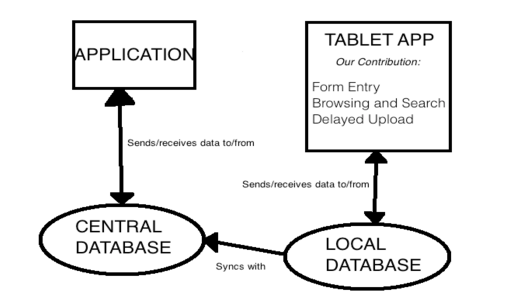
\includegraphics[width=4in,height=3in]{Diagram1.png}
\end{figure}




\clearpage\section[SYSTEM ARCHITECTURE]{\selectlanguage{english}\rmfamily\bfseries\color{black}
SYSTEM ARCHITECTURE}
\subsection[Architectural Design]{\selectlanguage{english}\rmfamily\bfseries\color{black}
Architectural Design}
{\selectlanguage{english}\rmfamily\color{black}
Develop a modular program structure and explain the relationships between the modules to
achieve the complete functionality of the system. This is a high level overview of how
Software Design Document
3
responsibilities of the system we repartitioned and then assigned to subsystems. Identify each
high level subsystem and the roles or responsibilities assigned to it. Describe how these
subsystems collaboratewith each otherin ordertoachievethedesiredfunctionality. Dont go
into too much detail about theindividual subsystems. The mainpurposeis to gain ageneral
understanding of how andwhy thesystem was decomposed, and howthe individual parts
worktogether. Provideadiagram showingthemajor subsystems anddatarepositories and
their interconnections. Describethediagram if required.}

\subsection[Decomposition Description]{\selectlanguage{english}\rmfamily\bfseries\color{black}
Decomposition Description}
{\selectlanguage{english}\rmfamily\color{black}
Provideadecomposition of thesubsystems in thearchitectural design. Supplement with text
as needed. Youmay chooseto giveafunctional description or an object­orienteddescription. For a functional description, put top­level data flow diagram (DFD) and structural
decomposition diagrams. For an OO description, put subsystem model, object diagrams, generalization hierarchy diagram(s) (if any), aggregation hierarchy diagram(s) (if any),
interface specifications, andsequence diagrams here.}

\subsection[Decomposition Description]{\selectlanguage{english}\rmfamily\bfseries\color{black}
Decomposition Description}
{\selectlanguage{english}\rmfamily\color{black}
Discuss the rationale for selecting the architecture described in 3.1 including critical issues
and trade/offs that were considered. You may discuss other architectures that were
considered, provided that you explain why you didnt choose them.
}

\clearpage\section[DATA DESIGN]{\selectlanguage{english}\rmfamily\bfseries\color{black}
DATA DESIGN}
\subsection[Data Description]{\selectlanguage{english}\rmfamily\bfseries\color{black}
Data Description}
{\selectlanguage{english}\rmfamily\color{black}
Explain howtheinformation domain of your system is transformedinto data structures. Describehowthemajor dataor system entities arestored, processedandorganized. List any
databases or datastorage items.
}

\subsection[Data Dictionary]{\selectlanguage{english}\rmfamily\bfseries\color{black}
Data Dictionary}
{\selectlanguage{english}\rmfamily\color{black}
Explain how the information domain of your system is transformedinto data structures. Describehowthemajor dataor system entities a restored, processed and organized. List any
databases or dat astorage items.
}


%\clearpage\section[DATA MODELING]{\selectlanguage{english}\rmfamily\bfseries\color{black}
%DATA MODELING}

\clearpage\section[COMPONENT DESIGN]{\selectlanguage{english}\rmfamily\bfseries\color{black}
COMPONENT DESIGN}
{\selectlanguage{english}\rmfamily\color{black}
In this section, we take acloserlookat what each component does in amoresystematicway. If
SoftwareDesignDocument
4
yougaveafunctional description insection 3.2, provideasummary of your algorithm for each
function listedin 3.2inprocedural description language (PDL) or pseudocode. If yougavean
OOdescription, summarize each object memberfunction for all theobjects listedin 3.2inPDL
or pseudocode. Describeany local datawhen necessary.
}


\clearpage\section{Human Interface Design}

\subsection[Overview of User Interface]{\selectlanguage{english}\rmfamily\bfseries\color{black}
Overview of User Interface}
{\selectlanguage{english}\rmfamily\color{black}
Describethefunctionality of thesystem from the users perspective. Explain howtheuser
will be able to use your system to complete all the expected features and the feedback
information that will bedisplayedfor theuser.
}
\subsection[Screen Images]{\selectlanguage{english}\rmfamily\bfseries\color{black}
Screen Images}
{\selectlanguage{english}\rmfamily\color{black}
Display screenshots showingtheinterfacefrom theusers perspective. Thesecan be handdrawn
or youcan use an automateddrawing tool. Just make them as accurateas possible.
(Graph paper workswell.)
}
\subsection[Screen Objects and Actions]{\selectlanguage{english}\rmfamily\bfseries\color{black}
Screen Objects and Actions}
{\selectlanguage{english}\rmfamily\color{black}
A discussion of screen objects andactions associatedwith thoseobjects.
}
\clearpage\section[APPENDIX A. ]{\selectlanguage{english}\rmfamily\bfseries\color{black}
APPENDIX A. \ Example Screens}

\bigskip

{\selectlanguage{english}\itshape\color{black}
Include copies of specifications, mockups, prototypes, etc. supplied or
derived from the customer. \ Appendices are labeled A, B, {\dots}n.
\ \ Reference each appendix as appropriate in the text of the document.
}

{\selectlanguage{english}\color{black}
\foreignlanguage{english}{\ }\foreignlanguage{english}{[ insert appendix
A here ]}}




\bigskip
\end{document}
